\begin{frame}[standout]

    Bases de données orientées graphe

    \note{
        Cette famille part des relations entre les entités.
        Elle est particulièrement intéressante lorsque les parcours dans
        le réseau sont aussi importants que les données elles-mêmes.
    }

\end{frame}

\begin{frame}{Caractéristiques des bases de données graphe}

    \begin{definitionbox}
        Dans une base de données graphe, les données sont organisées en \textbf{nœuds}, \textbf{liens} et \textbf{propriétés} qui permettent de modéliser des relations complexes et dynamiques entre les entités. Les \textbf{nœuds} représentent les entités, les \textbf{liens} représentent les relations entre ces nœuds, et les \textbf{propriétés} fournissent des informations supplémentaires sur les nœuds et les liens.
    \end{definitionbox}

    \begin{noteblock}
        \begin{itemize}
            \item Représentation des relations complexes entre les données.
            \item Optimisé pour les requêtes de lecture et les opérations relationnelles.
        \end{itemize}
        % $\Longrightarrow$ Idéal pour des applications nécessitant des relations complexes et dynamiques entre les données.
        $\hookrightarrow$ Idéal pour des applications nécessitant des relations complexes et dynamiques entre les données.
    \end{noteblock}

    \note{
        Un nœud représente une entité, une relation représente un lien orienté
        ou non, et les propriétés décrivent les deux. L'intérêt est de parcourir
        naturellement plusieurs niveaux de relations sans reconstruire de nombreuses
        jointures. Donner un exemple simple avec des personnes et leurs amis.
    }
\end{frame}

\begin{frame}{Bases de données graphe}
    \begin{figure}[htb]
        \centering
        \begin{tikzpicture}
            \node[minimum width=3cm, minimum height=2cm] at (0, 0) {\includesvg[height=1cm]{img/db/neo4j.svg}};
            \node[minimum width=3cm, minimum height=2cm] at (4, 0) {\includesvg[height=0.8cm]{img/db/arangodb.svg}};
            \node[minimum width=3cm, minimum height=2cm] at (0, -3) {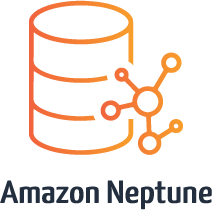
\includegraphics[height=1.3cm]{img/db/aws-neptune.png}};
            \node[minimum width=3cm, minimum height=2cm] at (4, -3) {\includesvg[height=1.3cm]{img/db/orientdb.svg}};
        \end{tikzpicture}
    \end{figure}

    \note{
        Neo4j est spécialisé dans le graphe de propriétés. ArangoDB propose
        plusieurs modèles, dont le graphe, et Neptune est un service managé.
        Le choix dépend des langages, du déploiement et des garanties recherchées.
    }
\end{frame}

\begin{frame}{Comment fonctionnent les bases de données graphe ?}

    \begin{figure}
        \centering
        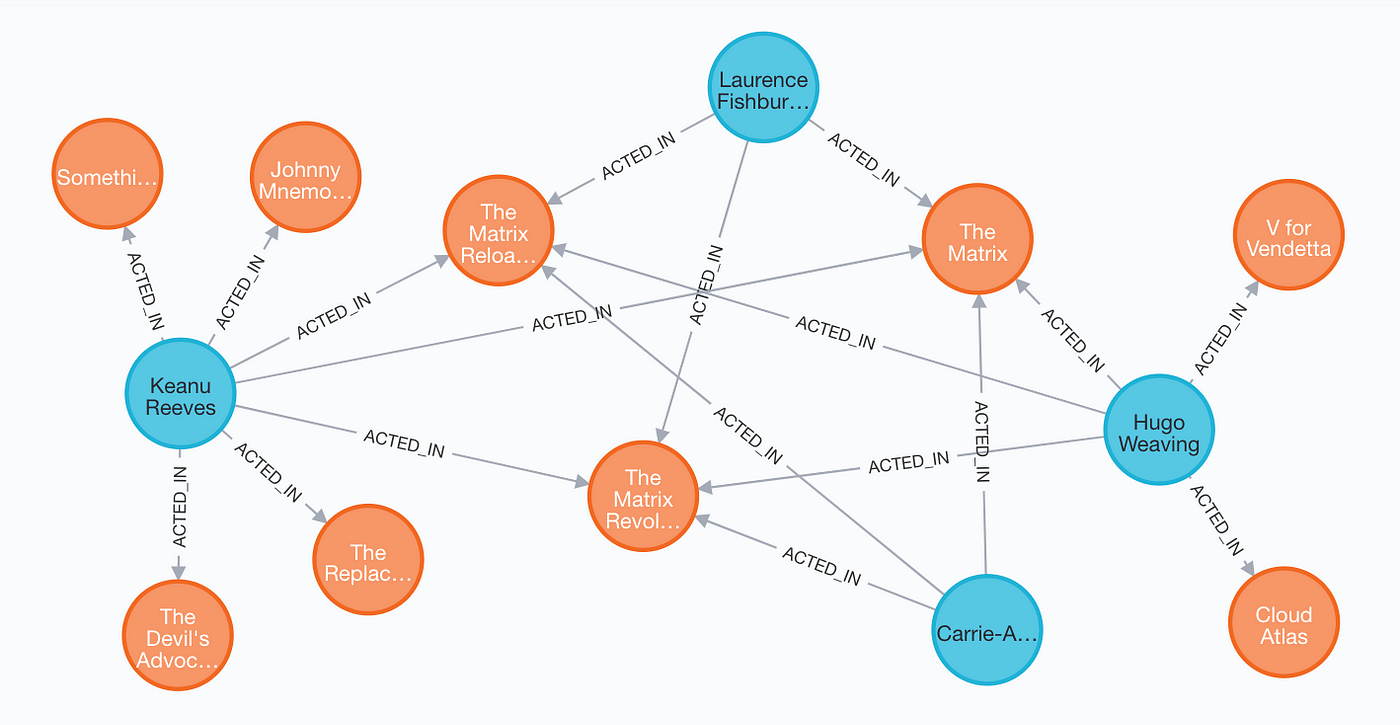
\includegraphics[width=0.8\textwidth]{img/neo4j-graph.png}
    \end{figure}

    \note{
        Lire le schéma comme un parcours : partir d'un nœud, suivre une relation,
        puis atteindre les voisins ou les voisins de voisins. C'est ce type de
        parcours qui rend les recommandations, la détection de fraude ou l'analyse
        de dépendances naturelles dans un graphe.
    }

\end{frame}

\begin{frame}{Cas d'usages des bases de données graphe}

    \begin{itemize}
        \item \textbf{Réseaux sociaux}\\
        $\hookrightarrow$ Modélisation des relations entre utilisateurs, amis, groupes, et interactions pour des recommandations et des analyses sociales.
        \vspace{0.3cm}

        \item \textbf{Systèmes de recommandation}\\
        $\hookrightarrow$ Analyse des préférences des utilisateurs et des relations entre produits pour fournir des recommandations personnalisées.
        \vspace{0.3cm}

        \item \textbf{Gestion des réseaux de télécommunications}\\
        $\hookrightarrow$ Modélisation des réseaux de télécommunications et des relations entre équipements pour optimiser les performances et la maintenance.
    \end{itemize}

    \note{
        Le graphe est pertinent quand la question porte sur les connexions :
        qui est relié à qui, par quel chemin, avec quelle dépendance ?
        Pour la fraude, on recherche des motifs dans les transactions.
        Pour les télécoms, on suit les équipements et les dépendances du réseau.
    }
\end{frame}

\begin{frame}{Avantages et inconvénients des bases de données graphe}
    \vfill
    \prosbox{
        \textbf{Avantages}
        \begin{itemize}
            \item Excellente performance pour les requêtes impliquant des relations complexes.
            \item Flexibilité pour modéliser des structures de données dynamiques.
        \end{itemize}
    }
    \vfill
    \pause
    \consbox{
        \textbf{Inconvénients}
        \begin{itemize}
            \item Moins efficace pour les opérations non liées aux relations.
            \item Complexité accrue pour les utilisateurs non familiers avec la modélisation en graphe.
        \end{itemize}
    }
    \vfill

    \note{
        Le gain est particulièrement visible pour les requêtes relationnelles
        et les parcours de plusieurs niveaux. En revanche, un graphe n'est pas
        automatiquement le meilleur choix pour des agrégations tabulaires simples
        ou des données sans relations significatives.
    }
\end{frame}
